\section{CXt\-Event\-Loop  Class Reference}
\label{classCXtEventLoop}\index{CXtEventLoop@{CXt\-Event\-Loop}}
{\tt \#include $<$CXt\-Event\-Loop.h$>$}

Inheritance diagram for CXt\-Event\-Loop::\begin{figure}[H]
\begin{center}
\leavevmode
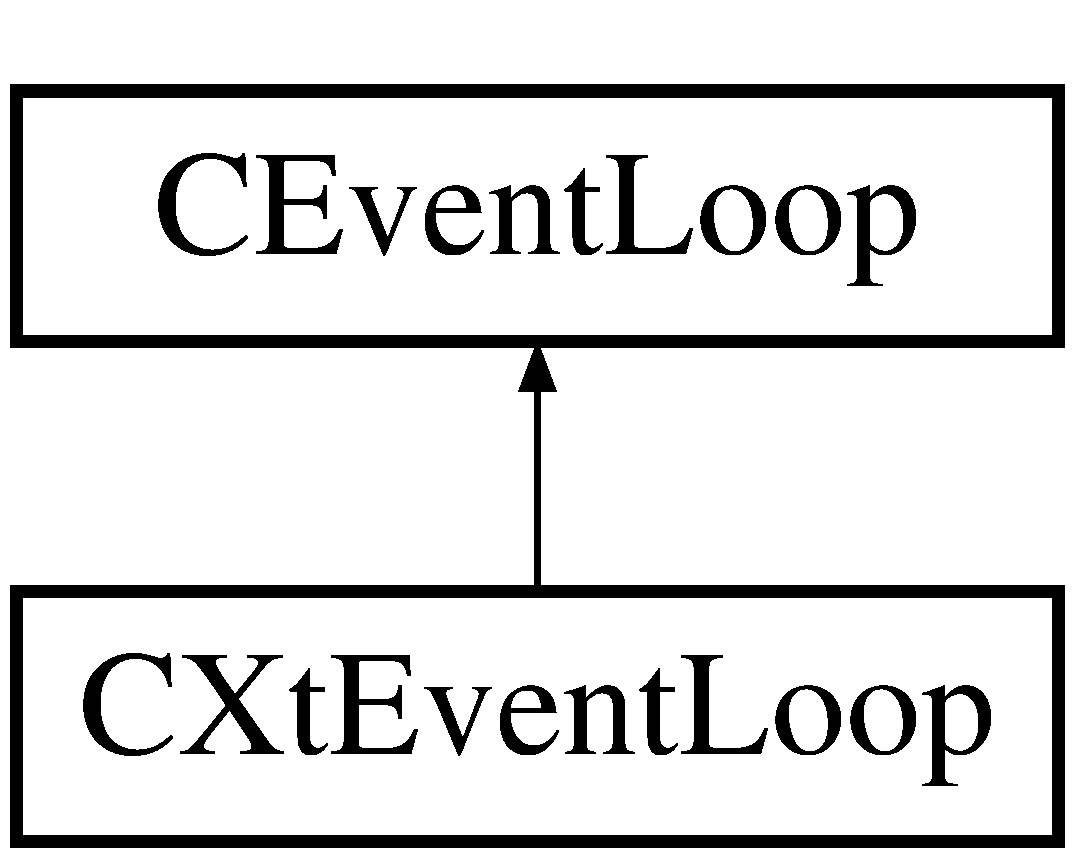
\includegraphics[height=2cm]{classCXtEventLoop}
\end{center}
\end{figure}
\subsection*{Public Methods}
\begin{CompactItemize}
\item 
{\bf CXt\-Event\-Loop} ()
\item 
virtual {\bf $\sim$CXt\-Event\-Loop} ()
\item 
Widget {\bf get\-Top\-Level} () const
\begin{CompactList}\small\item\em Returns the m\_\-Top\-Level member data.\item\end{CompactList}\item 
Xt\-App\-Context {\bf get\-App\-Context} () const
\begin{CompactList}\small\item\em Returns the application context.\item\end{CompactList}\item 
Xrm\-Option\-Desc\-Rec $\ast$ {\bf get\-Option\-Table} () const
\begin{CompactList}\small\item\em Returs a pointer to the option table.\item\end{CompactList}\item 
char $\ast$$\ast$ {\bf get\-Fallback\-Resources} () const
\begin{CompactList}\small\item\em Returns a pointer to the fallback resource list.\item\end{CompactList}\item 
string {\bf get\-Application\-Class} () const
\begin{CompactList}\small\item\em Returns the application class name.\item\end{CompactList}\item 
unsigned int {\bf get\-Option\-Count} () const
\begin{CompactList}\small\item\em Returns the number of options in the Option list.\item\end{CompactList}\item 
void {\bf exit} ()
\end{CompactItemize}
\subsection*{Protected Methods}
\begin{CompactItemize}
\item 
void {\bf set\-Top\-Level} (const Widget am\_\-Top\-Level)
\begin{CompactList}\small\item\em Set the value of the top level widget:.\item\end{CompactList}\item 
void {\bf set\-App\-Context} (Xt\-App\-Context new\-Context)
\begin{CompactList}\small\item\em Sets a new value for the application context.\item\end{CompactList}\item 
void {\bf set\-Option\-Table} (Xrm\-Option\-Desc\-Rec $\ast$p\-Table)
\begin{CompactList}\small\item\em Set a new option table pointer.\item\end{CompactList}\item 
void {\bf set\-Fallback\-Resources} (char $\ast$$\ast$resources)
\begin{CompactList}\small\item\em Set new fallback resource list.\item\end{CompactList}\item 
void {\bf set\-Application\-Class} (const string \&Class\-Name)
\begin{CompactList}\small\item\em Set a new application class string.\item\end{CompactList}\item 
void {\bf set\-Option\-Count} (unsigned int n\-Count)
\begin{CompactList}\small\item\em Set the number of items in the option list.\item\end{CompactList}\item 
virtual Widget {\bf Initialize\-Application} (int \&argc, char $\ast$$\ast$argv)
\item 
virtual void {\bf Setup\-Application\-Resources} (Widget Top\-Level)
\item 
virtual void {\bf Setup\-Widget\-Tree} (Widget Top\-Level)
\end{CompactItemize}
\subsection*{Private Methods}
\begin{CompactItemize}
\item 
virtual int {\bf operator()} (int argc, char $\ast$$\ast$argv)
\item 
{\bf CXt\-Event\-Loop} (const CXt\-Event\-Loop \&a\-CXt\-Event\-Loop)
\item 
CXt\-Event\-Loop \& {\bf operator=} (const CXt\-Event\-Loop \&a\-CXt\-Event\-Loop)
\item 
int {\bf operator==} (const CXt\-Event\-Loop \&a\-CXt\-Event\-Loop) const
\end{CompactItemize}
\subsection*{Private Attributes}
\begin{CompactItemize}
\item 
Widget {\bf m\_\-Top\-Level}
\item 
Xt\-App\-Context {\bf m\_\-App\-Context}
\begin{CompactList}\small\item\em Xt application context.\item\end{CompactList}\item 
Xrm\-Option\-Desc\-Rec $\ast$ {\bf m\_\-p\-Option\-Table}
\begin{CompactList}\small\item\em Command line option table (optional).\item\end{CompactList}\item 
unsigned int {\bf m\_\-n\-Option\-Count}
\begin{CompactList}\small\item\em Number of options.\item\end{CompactList}\item 
char $\ast$$\ast$ {\bf m\_\-ppc\-Fallback\-Resources}
\begin{CompactList}\small\item\em Application fall back resourcelist.\item\end{CompactList}\item 
string {\bf m\_\-s\-Class}
\begin{CompactList}\small\item\em Application class.\item\end{CompactList}\item 
bool {\bf m\_\-f\-Exit}
\begin{CompactList}\small\item\em TRUE when supposed to exit.\item\end{CompactList}\end{CompactItemize}


\subsection{Detailed Description}
Encapsulates an occurance of an Xt event loop.  The main loop synchronizes the event loop thread with the application each pass through the  Xt event loop e.g. the event loop looks like:

while(1) \{ Xt\-Get\-Event() Lock\-Mutex() Xt\-Dispatch\-Event(); Unlock\-Mutex(); yield(); // Let someone else run. \}

This implies that work procedures and timer procs are also synchonrized to the application. Note that this synchronization can be costly if there are work procedures continuously active. 



Definition at line 328 of file CXt\-Event\-Loop.h.

\subsection{Constructor \& Destructor Documentation}
\index{CXtEventLoop@{CXt\-Event\-Loop}!CXtEventLoop@{CXtEventLoop}}
\index{CXtEventLoop@{CXtEventLoop}!CXtEventLoop@{CXt\-Event\-Loop}}
\subsubsection{\setlength{\rightskip}{0pt plus 5cm}CXt\-Event\-Loop::CXt\-Event\-Loop ()}\label{classCXtEventLoop_a0}


The constructor is essentially a no-op. The base class already is checking for duplication of the singleton. We'll just let the exception pass up and through us  satisfying the condition that if an exception fires we prevent full construction.

The real work of initializing the Xt application is done in operator(), when we have a thread context of our own. 

Definition at line 314 of file CXt\-Event\-Loop.cpp.

References FALSE.\index{CXtEventLoop@{CXt\-Event\-Loop}!~CXtEventLoop@{$\sim$CXtEventLoop}}
\index{~CXtEventLoop@{$\sim$CXtEventLoop}!CXtEventLoop@{CXt\-Event\-Loop}}
\subsubsection{\setlength{\rightskip}{0pt plus 5cm}CXt\-Event\-Loop::$\sim$CXt\-Event\-Loop ()\hspace{0.3cm}{\tt  [virtual]}}\label{classCXtEventLoop_a1}


In theory the application specific code will destroy all application data and objects including the Xt application context and therefore this function is also a no-op.

Subclasses should either replace/supplement this or tear down the Xt stuff prior to destruction. 

Definition at line 334 of file CXt\-Event\-Loop.cpp.\index{CXtEventLoop@{CXt\-Event\-Loop}!CXtEventLoop@{CXtEventLoop}}
\index{CXtEventLoop@{CXtEventLoop}!CXtEventLoop@{CXt\-Event\-Loop}}
\subsubsection{\setlength{\rightskip}{0pt plus 5cm}CXt\-Event\-Loop::CXt\-Event\-Loop (const CXt\-Event\-Loop \& {\em a\-CXt\-Event\-Loop})\hspace{0.3cm}{\tt  [private]}}\label{classCXtEventLoop_c1}


Copy construction, assignment and equality comparison are invalid and hence declared privatge and not implemented. 

\subsection{Member Function Documentation}
\index{CXtEventLoop@{CXt\-Event\-Loop}!exit@{exit}}
\index{exit@{exit}!CXtEventLoop@{CXt\-Event\-Loop}}
\subsubsection{\setlength{\rightskip}{0pt plus 5cm}void CXt\-Event\-Loop::exit ()\hspace{0.3cm}{\tt  [inline]}}\label{classCXtEventLoop_a8}




Definition at line 427 of file CXt\-Event\-Loop.h.

References m\_\-f\-Exit, and TRUE.\index{CXtEventLoop@{CXt\-Event\-Loop}!getAppContext@{getAppContext}}
\index{getAppContext@{getAppContext}!CXtEventLoop@{CXt\-Event\-Loop}}
\subsubsection{\setlength{\rightskip}{0pt plus 5cm}Xt\-App\-Context CXt\-Event\-Loop::get\-App\-Context () const\hspace{0.3cm}{\tt  [inline]}}\label{classCXtEventLoop_a3}


Returns the application context.



Definition at line 367 of file CXt\-Event\-Loop.h.

References m\_\-App\-Context.\index{CXtEventLoop@{CXt\-Event\-Loop}!getApplicationClass@{getApplicationClass}}
\index{getApplicationClass@{getApplicationClass}!CXtEventLoop@{CXt\-Event\-Loop}}
\subsubsection{\setlength{\rightskip}{0pt plus 5cm}string CXt\-Event\-Loop::get\-Application\-Class () const\hspace{0.3cm}{\tt  [inline]}}\label{classCXtEventLoop_a6}


Returns the application class name.



Definition at line 382 of file CXt\-Event\-Loop.h.

References m\_\-s\-Class.\index{CXtEventLoop@{CXt\-Event\-Loop}!getFallbackResources@{getFallbackResources}}
\index{getFallbackResources@{getFallbackResources}!CXtEventLoop@{CXt\-Event\-Loop}}
\subsubsection{\setlength{\rightskip}{0pt plus 5cm}char$\ast$$\ast$ CXt\-Event\-Loop::get\-Fallback\-Resources () const\hspace{0.3cm}{\tt  [inline]}}\label{classCXtEventLoop_a5}


Returns a pointer to the fallback resource list.



Definition at line 377 of file CXt\-Event\-Loop.h.

References m\_\-ppc\-Fallback\-Resources.\index{CXtEventLoop@{CXt\-Event\-Loop}!getOptionCount@{getOptionCount}}
\index{getOptionCount@{getOptionCount}!CXtEventLoop@{CXt\-Event\-Loop}}
\subsubsection{\setlength{\rightskip}{0pt plus 5cm}unsigned int CXt\-Event\-Loop::get\-Option\-Count () const\hspace{0.3cm}{\tt  [inline]}}\label{classCXtEventLoop_a7}


Returns the number of options in the Option list.



Definition at line 387 of file CXt\-Event\-Loop.h.

References m\_\-n\-Option\-Count.\index{CXtEventLoop@{CXt\-Event\-Loop}!getOptionTable@{getOptionTable}}
\index{getOptionTable@{getOptionTable}!CXtEventLoop@{CXt\-Event\-Loop}}
\subsubsection{\setlength{\rightskip}{0pt plus 5cm}Xrm\-Option\-Desc\-Rec$\ast$ CXt\-Event\-Loop::get\-Option\-Table () const\hspace{0.3cm}{\tt  [inline]}}\label{classCXtEventLoop_a4}


Returs a pointer to the option table.



Definition at line 372 of file CXt\-Event\-Loop.h.

References m\_\-p\-Option\-Table.\index{CXtEventLoop@{CXt\-Event\-Loop}!getTopLevel@{getTopLevel}}
\index{getTopLevel@{getTopLevel}!CXtEventLoop@{CXt\-Event\-Loop}}
\subsubsection{\setlength{\rightskip}{0pt plus 5cm}Widget CXt\-Event\-Loop::get\-Top\-Level () const\hspace{0.3cm}{\tt  [inline]}}\label{classCXtEventLoop_a2}


Returns the m\_\-Top\-Level member data.



Definition at line 362 of file CXt\-Event\-Loop.h.

References m\_\-Top\-Level.\index{CXtEventLoop@{CXt\-Event\-Loop}!InitializeApplication@{InitializeApplication}}
\index{InitializeApplication@{InitializeApplication}!CXtEventLoop@{CXt\-Event\-Loop}}
\subsubsection{\setlength{\rightskip}{0pt plus 5cm}Widget CXt\-Event\-Loop::Initialize\-Application (int \& {\em argc}, char $\ast$$\ast$ {\em argv})\hspace{0.3cm}{\tt  [protected, virtual]}}\label{classCXtEventLoop_b6}


Called to initialize the X toolkit. Default behavior is to call Xt\-Appinit(), and return its result.

A typical implementation of a subclass will might setup an options table and call set\-Option\-Table and set\-Option\-Count, Override the default class name via set\-Application\-Class, and  fill in a set of fallback resources via set\-Fallback\-Resources 

Definition at line 354 of file CXt\-Event\-Loop.cpp.

References m\_\-App\-Context, m\_\-n\-Option\-Count, m\_\-p\-Option\-Table, m\_\-ppc\-Fallback\-Resources, m\_\-s\-Class, and m\_\-Top\-Level.

Referenced by operator()().\index{CXtEventLoop@{CXt\-Event\-Loop}!operator()@{operator()}}
\index{operator()@{operator()}!CXtEventLoop@{CXt\-Event\-Loop}}
\subsubsection{\setlength{\rightskip}{0pt plus 5cm}int CXt\-Event\-Loop::operator() (int {\em argc}, char $\ast$$\ast$ {\em argv})\hspace{0.3cm}{\tt  [private, virtual]}}\label{classCXtEventLoop_c0}


Entry point for the Xt event loop thread. The initialization functions are called to allow the application to set up the application widget set. After this is done, the event loop is entered. Each call of Xt\-Dispatch\-Event is bracketed by calls to lock/unlock the application serializatio mutex.

Note that throughout the entire initialization of the Xt, the global mutex is held. 

Implements {\bf CEvent\-Loop} {\rm (p.\,\pageref{classCEventLoop_c0})}.

Definition at line 420 of file CXt\-Event\-Loop.cpp.

References CApplication\-Serializer::get\-Instance(), Initialize\-Application(), CThread\-Recursive\-Mutex::Lock(), m\_\-App\-Context, m\_\-f\-Exit, m\_\-Top\-Level, Setup\-Application\-Resources(), Setup\-Widget\-Tree(), and CThread\-Recursive\-Mutex::Un\-Lock().\index{CXtEventLoop@{CXt\-Event\-Loop}!operator=@{operator=}}
\index{operator=@{operator=}!CXtEventLoop@{CXt\-Event\-Loop}}
\subsubsection{\setlength{\rightskip}{0pt plus 5cm}CXt\-Event\-Loop\& CXt\-Event\-Loop::operator= (const CXt\-Event\-Loop \& {\em a\-CXt\-Event\-Loop})\hspace{0.3cm}{\tt  [private]}}\label{classCXtEventLoop_c2}


\index{CXtEventLoop@{CXt\-Event\-Loop}!operator==@{operator==}}
\index{operator==@{operator==}!CXtEventLoop@{CXt\-Event\-Loop}}
\subsubsection{\setlength{\rightskip}{0pt plus 5cm}int CXt\-Event\-Loop::operator== (const CXt\-Event\-Loop \& {\em a\-CXt\-Event\-Loop}) const\hspace{0.3cm}{\tt  [private]}}\label{classCXtEventLoop_c3}


\index{CXtEventLoop@{CXt\-Event\-Loop}!setAppContext@{setAppContext}}
\index{setAppContext@{setAppContext}!CXtEventLoop@{CXt\-Event\-Loop}}
\subsubsection{\setlength{\rightskip}{0pt plus 5cm}void CXt\-Event\-Loop::set\-App\-Context (Xt\-App\-Context {\em new\-Context})\hspace{0.3cm}{\tt  [inline, protected]}}\label{classCXtEventLoop_b1}


Sets a new value for the application context.



Definition at line 398 of file CXt\-Event\-Loop.h.

References m\_\-App\-Context.\index{CXtEventLoop@{CXt\-Event\-Loop}!setApplicationClass@{setApplicationClass}}
\index{setApplicationClass@{setApplicationClass}!CXtEventLoop@{CXt\-Event\-Loop}}
\subsubsection{\setlength{\rightskip}{0pt plus 5cm}void CXt\-Event\-Loop::set\-Application\-Class (const string \& {\em Class\-Name})\hspace{0.3cm}{\tt  [inline, protected]}}\label{classCXtEventLoop_b4}


Set a new application class string.



Definition at line 411 of file CXt\-Event\-Loop.h.

References m\_\-s\-Class.\index{CXtEventLoop@{CXt\-Event\-Loop}!setFallbackResources@{setFallbackResources}}
\index{setFallbackResources@{setFallbackResources}!CXtEventLoop@{CXt\-Event\-Loop}}
\subsubsection{\setlength{\rightskip}{0pt plus 5cm}void CXt\-Event\-Loop::set\-Fallback\-Resources (char $\ast$$\ast$ {\em resources})\hspace{0.3cm}{\tt  [inline, protected]}}\label{classCXtEventLoop_b3}


Set new fallback resource list.

\begin{Desc}
\item[{\bf Bug: }]\par
 May want to do a copy in instead of pointer copy.\end{Desc}
 

Definition at line 407 of file CXt\-Event\-Loop.h.

References m\_\-ppc\-Fallback\-Resources.\index{CXtEventLoop@{CXt\-Event\-Loop}!setOptionCount@{setOptionCount}}
\index{setOptionCount@{setOptionCount}!CXtEventLoop@{CXt\-Event\-Loop}}
\subsubsection{\setlength{\rightskip}{0pt plus 5cm}void CXt\-Event\-Loop::set\-Option\-Count (unsigned int {\em n\-Count})\hspace{0.3cm}{\tt  [inline, protected]}}\label{classCXtEventLoop_b5}


Set the number of items in the option list.



Definition at line 415 of file CXt\-Event\-Loop.h.

References m\_\-n\-Option\-Count.\index{CXtEventLoop@{CXt\-Event\-Loop}!setOptionTable@{setOptionTable}}
\index{setOptionTable@{setOptionTable}!CXtEventLoop@{CXt\-Event\-Loop}}
\subsubsection{\setlength{\rightskip}{0pt plus 5cm}void CXt\-Event\-Loop::set\-Option\-Table (Xrm\-Option\-Desc\-Rec $\ast$ {\em p\-Table})\hspace{0.3cm}{\tt  [inline, protected]}}\label{classCXtEventLoop_b2}


Set a new option table pointer.



Definition at line 402 of file CXt\-Event\-Loop.h.

References m\_\-p\-Option\-Table.\index{CXtEventLoop@{CXt\-Event\-Loop}!setTopLevel@{setTopLevel}}
\index{setTopLevel@{setTopLevel}!CXtEventLoop@{CXt\-Event\-Loop}}
\subsubsection{\setlength{\rightskip}{0pt plus 5cm}void CXt\-Event\-Loop::set\-Top\-Level (const Widget {\em am\_\-Top\-Level})\hspace{0.3cm}{\tt  [inline, protected]}}\label{classCXtEventLoop_b0}


Set the value of the top level widget:.



Definition at line 393 of file CXt\-Event\-Loop.h.

References m\_\-Top\-Level.\index{CXtEventLoop@{CXt\-Event\-Loop}!SetupApplicationResources@{SetupApplicationResources}}
\index{SetupApplicationResources@{SetupApplicationResources}!CXtEventLoop@{CXt\-Event\-Loop}}
\subsubsection{\setlength{\rightskip}{0pt plus 5cm}void CXt\-Event\-Loop::Setup\-Application\-Resources (Widget {\em Top\-Level})\hspace{0.3cm}{\tt  [protected, virtual]}}\label{classCXtEventLoop_b7}


Called from operator() to process the resource database. Since the resource database requires definitions which are application specific but is not actually  required, the default behavior is to do nothing.

Normal applications will override this member toset  up resource definition structures, invoke Xt\-Get\-Application\-Resrouces() to retrieve the actual values from the resource database and validity check them.

$\backslash$ 

Definition at line 386 of file CXt\-Event\-Loop.cpp.

Referenced by operator()().\index{CXtEventLoop@{CXt\-Event\-Loop}!SetupWidgetTree@{SetupWidgetTree}}
\index{SetupWidgetTree@{SetupWidgetTree}!CXtEventLoop@{CXt\-Event\-Loop}}
\subsubsection{\setlength{\rightskip}{0pt plus 5cm}void CXt\-Event\-Loop::Setup\-Widget\-Tree (Widget {\em Top\-Level})\hspace{0.3cm}{\tt  [protected, virtual]}}\label{classCXtEventLoop_b8}


operator() calls this function to set up the initial widget tree.

This is completely application specific. Most applications will require a widget tree in addition to the shell widget produced by Xt\-App\-Initialize(). This member should be overridden to produce this tree. 

Definition at line 401 of file CXt\-Event\-Loop.cpp.

Referenced by operator()().

\subsection{Member Data Documentation}
\index{CXtEventLoop@{CXt\-Event\-Loop}!m_AppContext@{m\_\-AppContext}}
\index{m_AppContext@{m\_\-AppContext}!CXtEventLoop@{CXt\-Event\-Loop}}
\subsubsection{\setlength{\rightskip}{0pt plus 5cm}Xt\-App\-Context CXt\-Event\-Loop::m\_\-App\-Context\hspace{0.3cm}{\tt  [private]}}\label{classCXtEventLoop_o1}


Xt application context.



Definition at line 336 of file CXt\-Event\-Loop.h.

Referenced by get\-App\-Context(), Initialize\-Application(), operator()(), and set\-App\-Context().\index{CXtEventLoop@{CXt\-Event\-Loop}!m_fExit@{m\_\-fExit}}
\index{m_fExit@{m\_\-fExit}!CXtEventLoop@{CXt\-Event\-Loop}}
\subsubsection{\setlength{\rightskip}{0pt plus 5cm}bool CXt\-Event\-Loop::m\_\-f\-Exit\hspace{0.3cm}{\tt  [private]}}\label{classCXtEventLoop_o6}


TRUE when supposed to exit.



Definition at line 342 of file CXt\-Event\-Loop.h.

Referenced by exit(), and operator()().\index{CXtEventLoop@{CXt\-Event\-Loop}!m_nOptionCount@{m\_\-nOptionCount}}
\index{m_nOptionCount@{m\_\-nOptionCount}!CXtEventLoop@{CXt\-Event\-Loop}}
\subsubsection{\setlength{\rightskip}{0pt plus 5cm}unsigned int CXt\-Event\-Loop::m\_\-n\-Option\-Count\hspace{0.3cm}{\tt  [private]}}\label{classCXtEventLoop_o3}


Number of options.



Definition at line 339 of file CXt\-Event\-Loop.h.

Referenced by get\-Option\-Count(), Initialize\-Application(), and set\-Option\-Count().\index{CXtEventLoop@{CXt\-Event\-Loop}!m_pOptionTable@{m\_\-pOptionTable}}
\index{m_pOptionTable@{m\_\-pOptionTable}!CXtEventLoop@{CXt\-Event\-Loop}}
\subsubsection{\setlength{\rightskip}{0pt plus 5cm}Xrm\-Option\-Desc\-Rec$\ast$ CXt\-Event\-Loop::m\_\-p\-Option\-Table\hspace{0.3cm}{\tt  [private]}}\label{classCXtEventLoop_o2}


Command line option table (optional).



Definition at line 338 of file CXt\-Event\-Loop.h.

Referenced by get\-Option\-Table(), Initialize\-Application(), and set\-Option\-Table().\index{CXtEventLoop@{CXt\-Event\-Loop}!m_ppcFallbackResources@{m\_\-ppcFallbackResources}}
\index{m_ppcFallbackResources@{m\_\-ppcFallbackResources}!CXtEventLoop@{CXt\-Event\-Loop}}
\subsubsection{\setlength{\rightskip}{0pt plus 5cm}char$\ast$$\ast$ CXt\-Event\-Loop::m\_\-ppc\-Fallback\-Resources\hspace{0.3cm}{\tt  [private]}}\label{classCXtEventLoop_o4}


Application fall back resourcelist.



Definition at line 340 of file CXt\-Event\-Loop.h.

Referenced by get\-Fallback\-Resources(), Initialize\-Application(), and set\-Fallback\-Resources().\index{CXtEventLoop@{CXt\-Event\-Loop}!m_sClass@{m\_\-sClass}}
\index{m_sClass@{m\_\-sClass}!CXtEventLoop@{CXt\-Event\-Loop}}
\subsubsection{\setlength{\rightskip}{0pt plus 5cm}string CXt\-Event\-Loop::m\_\-s\-Class\hspace{0.3cm}{\tt  [private]}}\label{classCXtEventLoop_o5}


Application class.



Definition at line 341 of file CXt\-Event\-Loop.h.

Referenced by get\-Application\-Class(), Initialize\-Application(), and set\-Application\-Class().\index{CXtEventLoop@{CXt\-Event\-Loop}!m_TopLevel@{m\_\-TopLevel}}
\index{m_TopLevel@{m\_\-TopLevel}!CXtEventLoop@{CXt\-Event\-Loop}}
\subsubsection{\setlength{\rightskip}{0pt plus 5cm}Widget CXt\-Event\-Loop::m\_\-Top\-Level\hspace{0.3cm}{\tt  [private]}}\label{classCXtEventLoop_o0}


m\_\-Top\-Level is the top level of the application's widget hierarchy. in order to use the Xm++ library it will be necessary to retrieve this and instantiate Widget object from it. 

Definition at line 335 of file CXt\-Event\-Loop.h.

Referenced by get\-Top\-Level(), Initialize\-Application(), operator()(), and set\-Top\-Level().

The documentation for this class was generated from the following files:\begin{CompactItemize}
\item 
{\bf CXt\-Event\-Loop.h}\item 
{\bf CXt\-Event\-Loop.cpp}\end{CompactItemize}
